\documentclass[12pt]{article}
\usepackage[T1]{fontenc}
\usepackage{latex_packages/pythontex}
\usepackage{atbegshi}
\usepackage{graphicx}
\usepackage{hyperref}
\AtBeginDocument{\AtBeginShipoutNext{\AtBeginShipoutDiscard}}

\begin{document} \noindent
\title{\Huge \textbf{Gamenter}}
\author{\textit{Tedeschini Luca,Preti Christian}}
\date{2021/22}
\maketitle \noindent
In questo documento verranno documentati 10 diversi \textit{benchmarks}, effettuati attraverso motore di ricerca \textit{Gamenter}, al fine di valutarne le peculiarità e la correttezza dei risultati.
\\ \\
Ogni \textit{benchmark} sarà strutturato in questo modo:

\begin{itemize}
	\item Query con rappresentazione umana, ad esempio: "Vorrei fare una ricerca per giochi, cercando le keyword \{$kw_1, kw_2, ..., kw_n$\} "
	
	\item Traduzione da linguaggio parlato a query language.

	\item Valutazione dei risultati.

\end{itemize}

\noindent La valutazione dei risultati terrà conto di 2 fattori:

\begin{itemize}
	\item Correttezza del risultato.
	\item Tempo di esecuzione della query.
\end{itemize} 

\noindent Di seguito, verranno illustrati alcuni esempi di query, seguendo la struttura sopra riportata. \\ \\
\textbf{P.S} In alcuni casi, è possibile che il ranking di alcuni giochi sia pari a 0, questo è dovuto a un mancato voto sul sito \url{https://www.metacritic.com}
\pagebreak

\paragraph{\LARGE{Query 1}} ~ \\ \\

\noindent \textbf{Keywords: } horizon \\
\textbf{Filters: } \{ \\ 
	\indent content True, \\
	\indent mark > 75 \\
\} \\\\
 	
\noindent 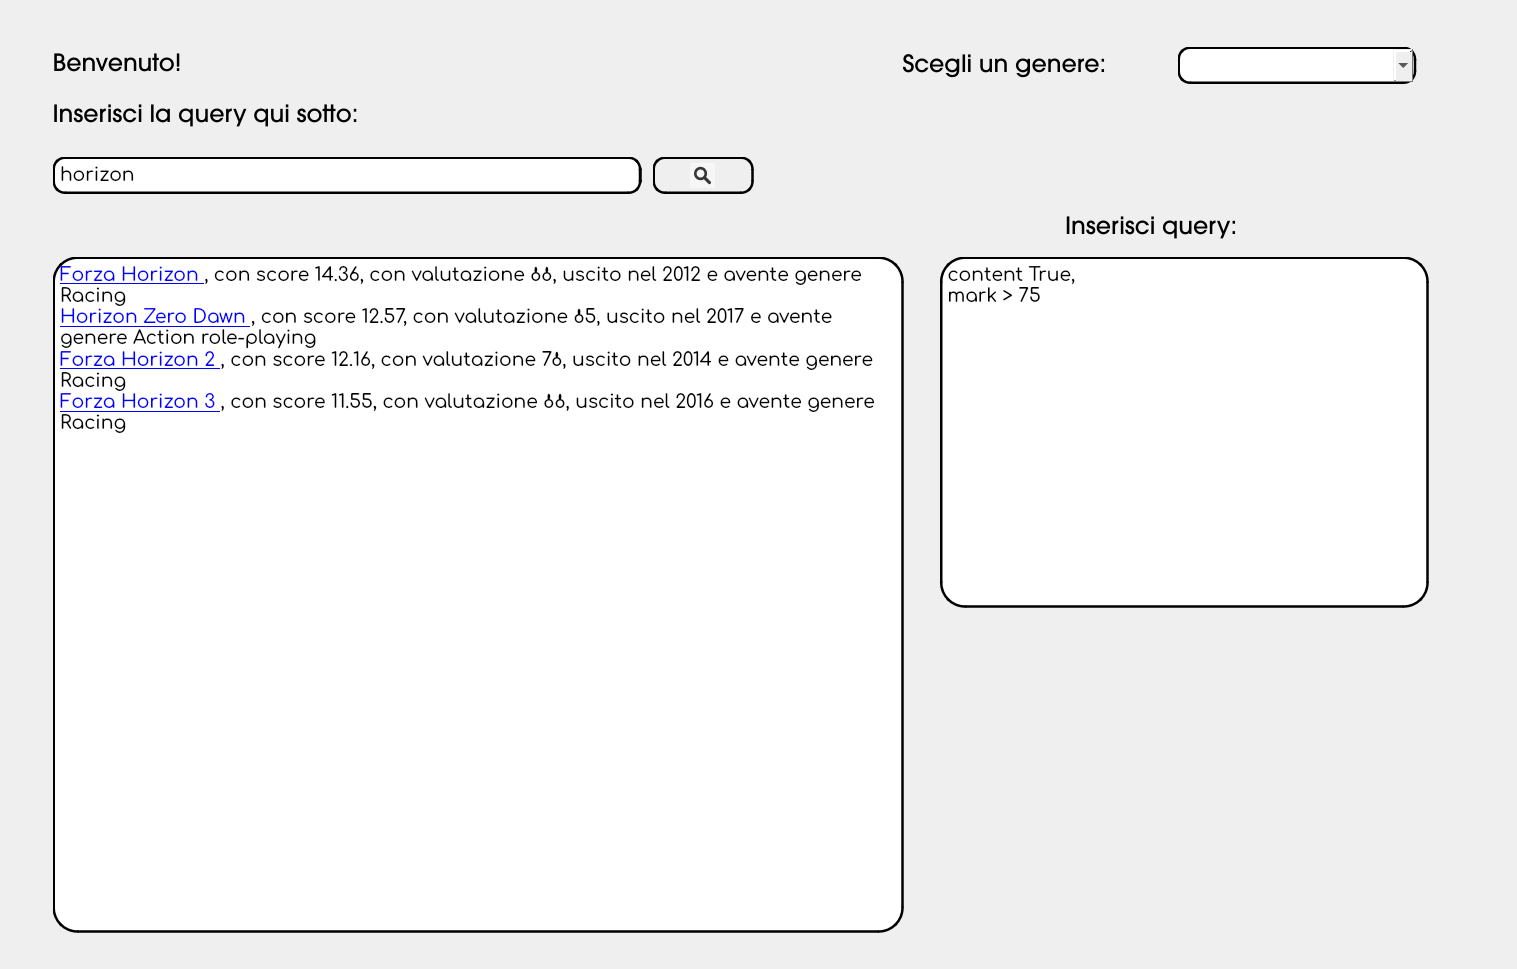
\includegraphics[width=100mm]{Immagini/Image1.png} \\
\textbf{Tempo di esecuzione:} 0.00965s \\
\textbf{Correttezza:} 100\% \pagebreak

\paragraph{\LARGE{Query 2}} ~ \\ \\

\noindent \textbf{Keywords: } Pokemon \\
\textbf{Filters: } \{ \\ \\
\indent year > 2010, \\
\indent year < 2016 \\
\} \\\\

\noindent 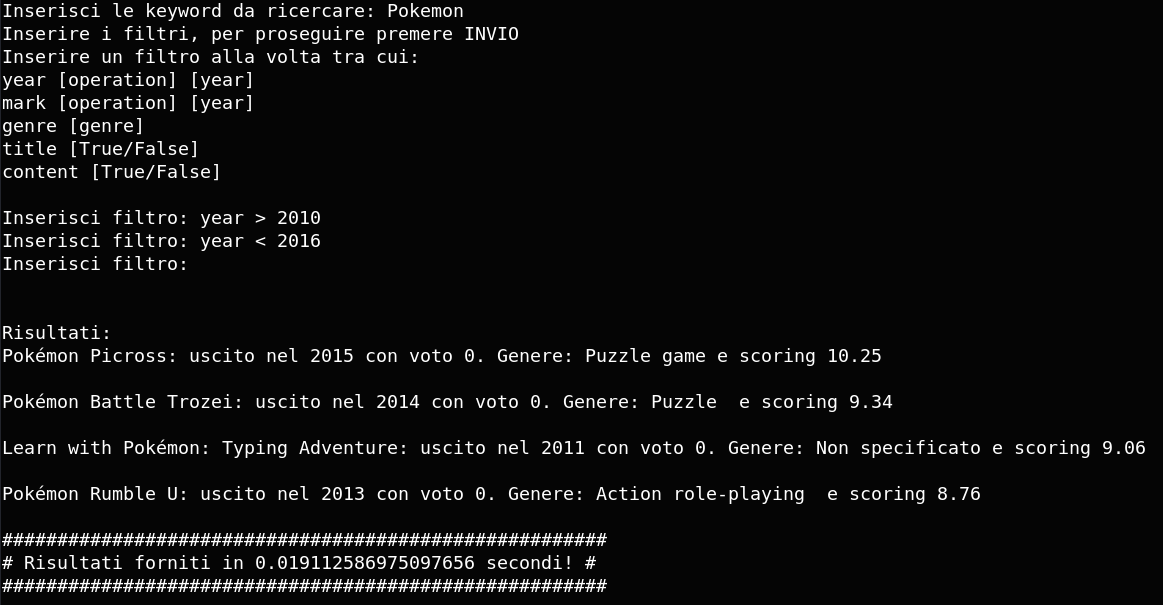
\includegraphics[width=100mm]{Immagini/Image2.png} \\
\textbf{Tempo di esecuzione:} 0.01911s \\
\textbf{Correttezza:} 100\% \pagebreak

\paragraph{\LARGE{Query 3}} ~ \\ \\

\noindent \textbf{Keywords: } super mario \\
\textbf{Filters: } \{ \\ \\
\indent year < 2020, \\
\indent year > 2013 \\
\indent content False \\
\} \\\\

\noindent 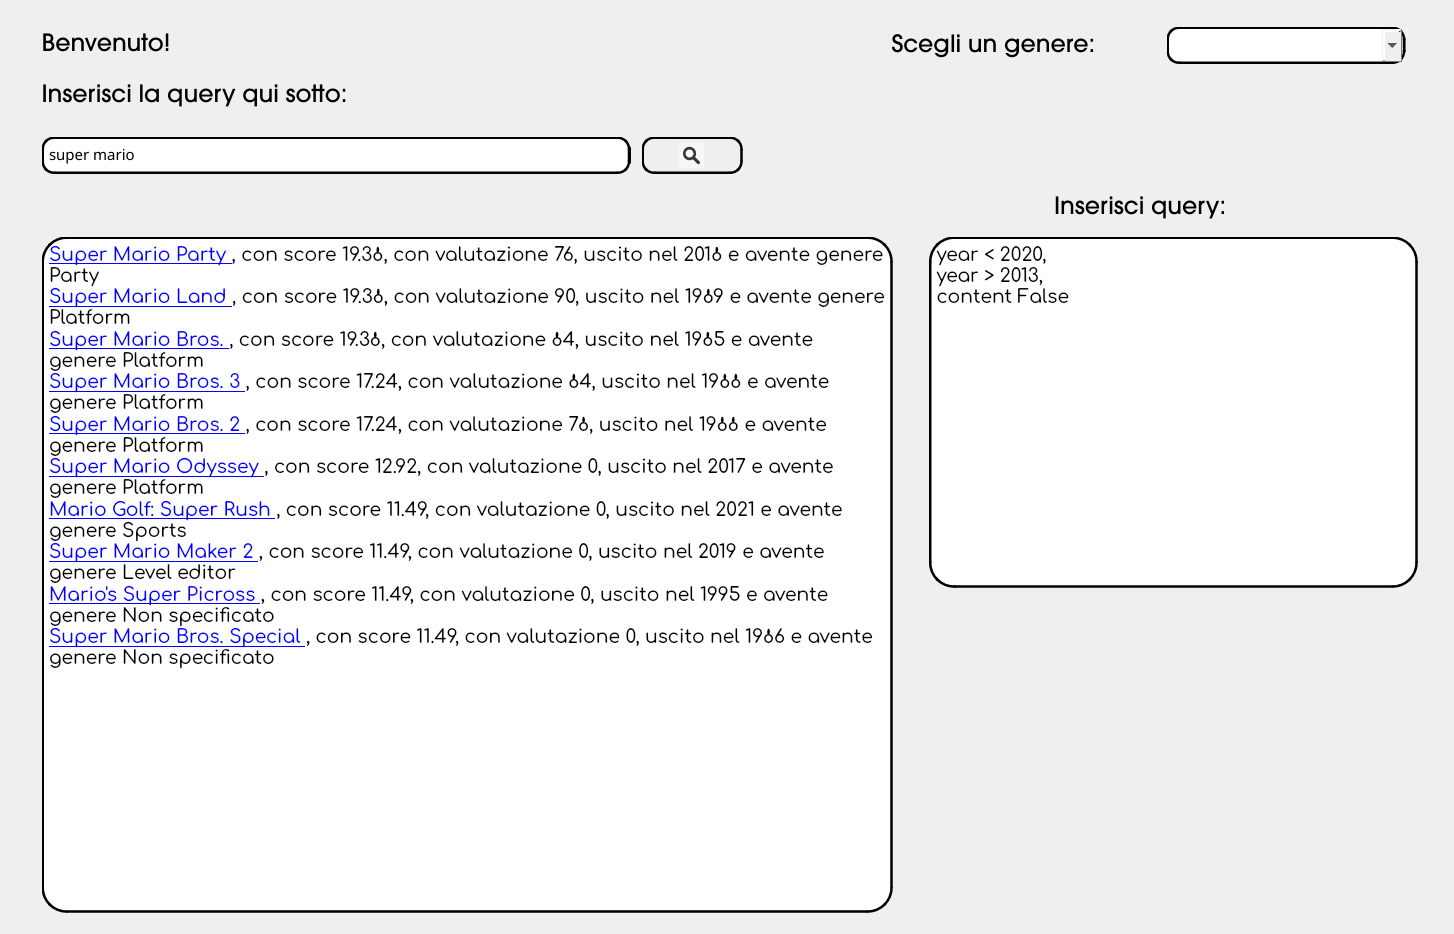
\includegraphics[width=100mm]{Immagini/Image3.png} \\
\textbf{Tempo di esecuzione:} 0.052491 \\
\textbf{Correttezza:} 100\% \pagebreak

\paragraph{Query 4} ~ \\ \\

\noindent \textbf{Keywords: } horizon \\
\textbf{Filters: } \{ \\ \\
\indent content True, \\
\indent mark > 75 \\
\} \\\\

\noindent 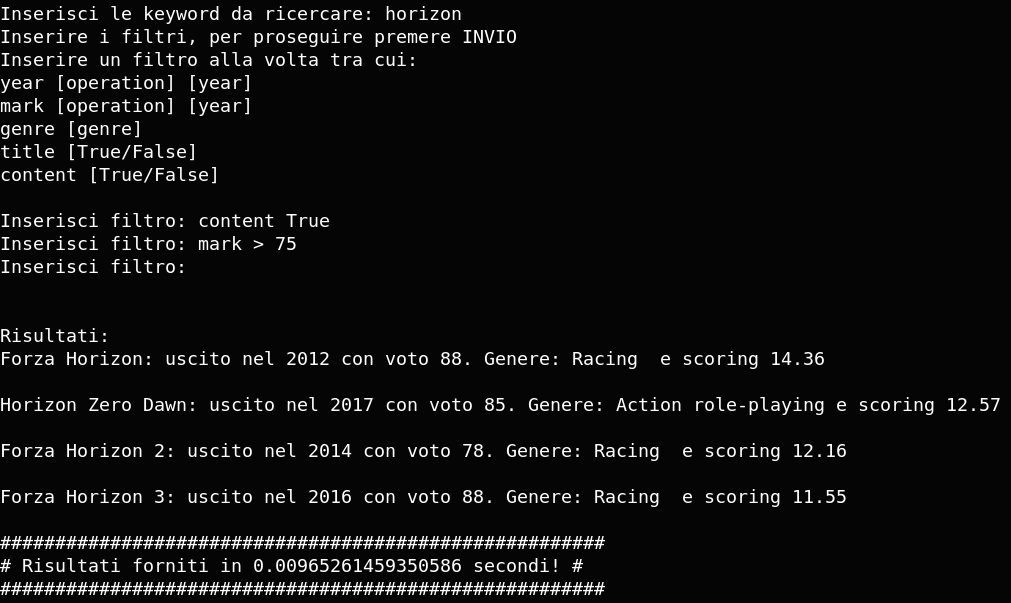
\includegraphics[width=100mm]{Immagini/Image4.png} \\
\textbf{Tempo di esecuzione:} 0.009652 \\
\textbf{Correttezza:} 100\% \pagebreak

\paragraph{Query 5} ~ \\ \\

\noindent \textbf{Keywords: } grand theft auto \\
\textbf{Filters: } \{ \\ \\
\indent mark > 80 \\
\} \\\\

\noindent 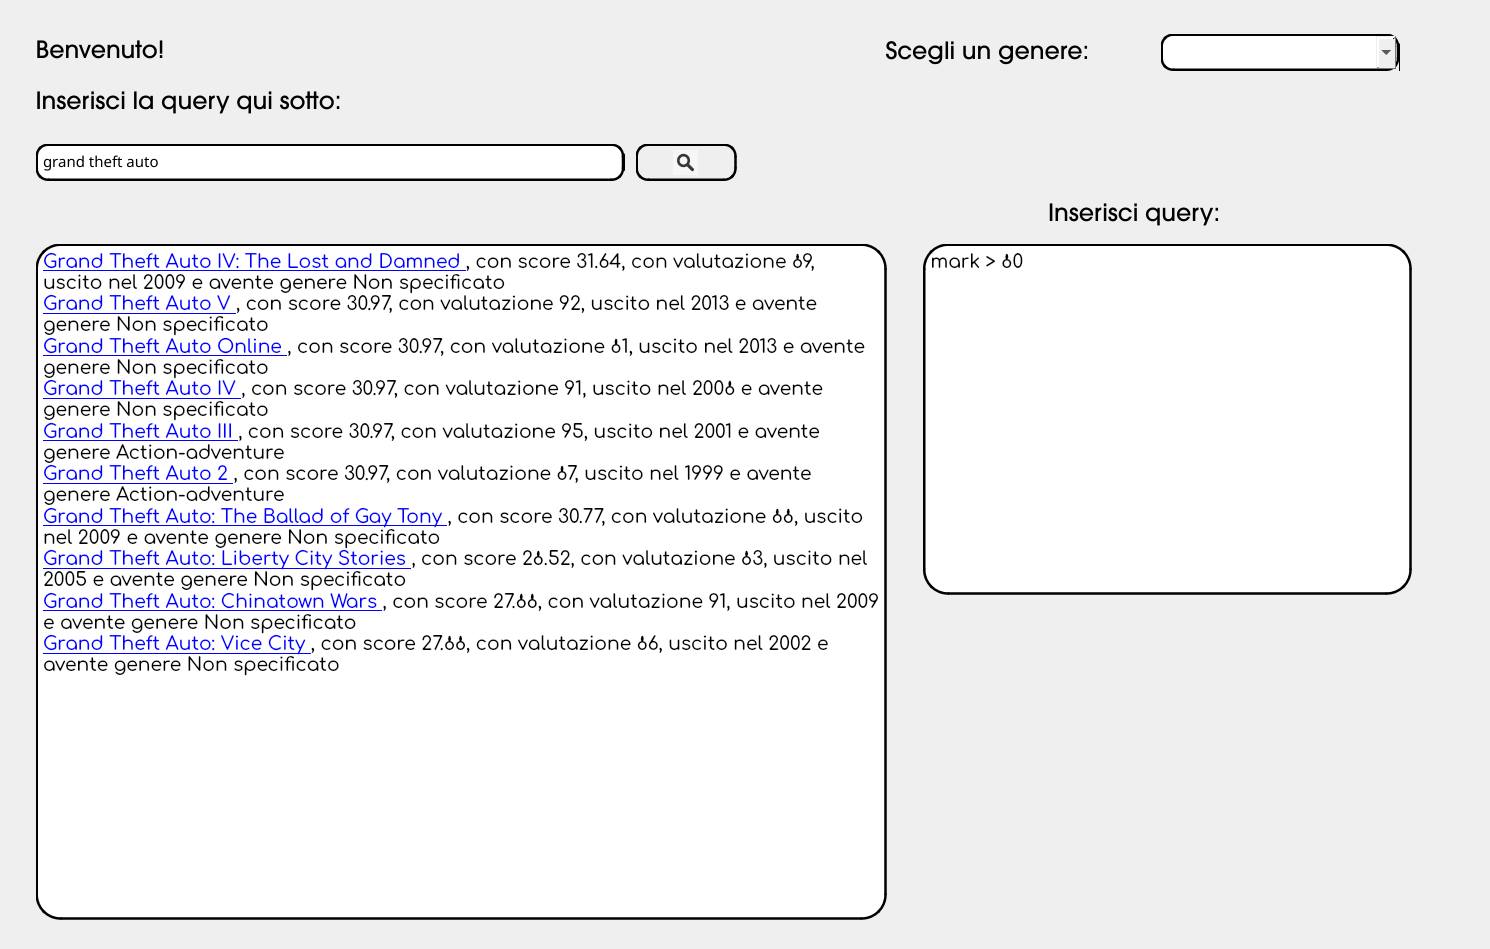
\includegraphics[width=100mm]{Immagini/Image5.png} \\
\textbf{Tempo di esecuzione:} 0.0077886 \\
\textbf{Correttezza:} 100\% \pagebreak

\paragraph{Query 6} ~ \\ \\

\noindent \textbf{Keywords: } Pokemon \\
\textbf{Filters: } \{ \\ \\
\indent year > 2010, \\
\indent year < 2016 \\
\} \\\\

\noindent 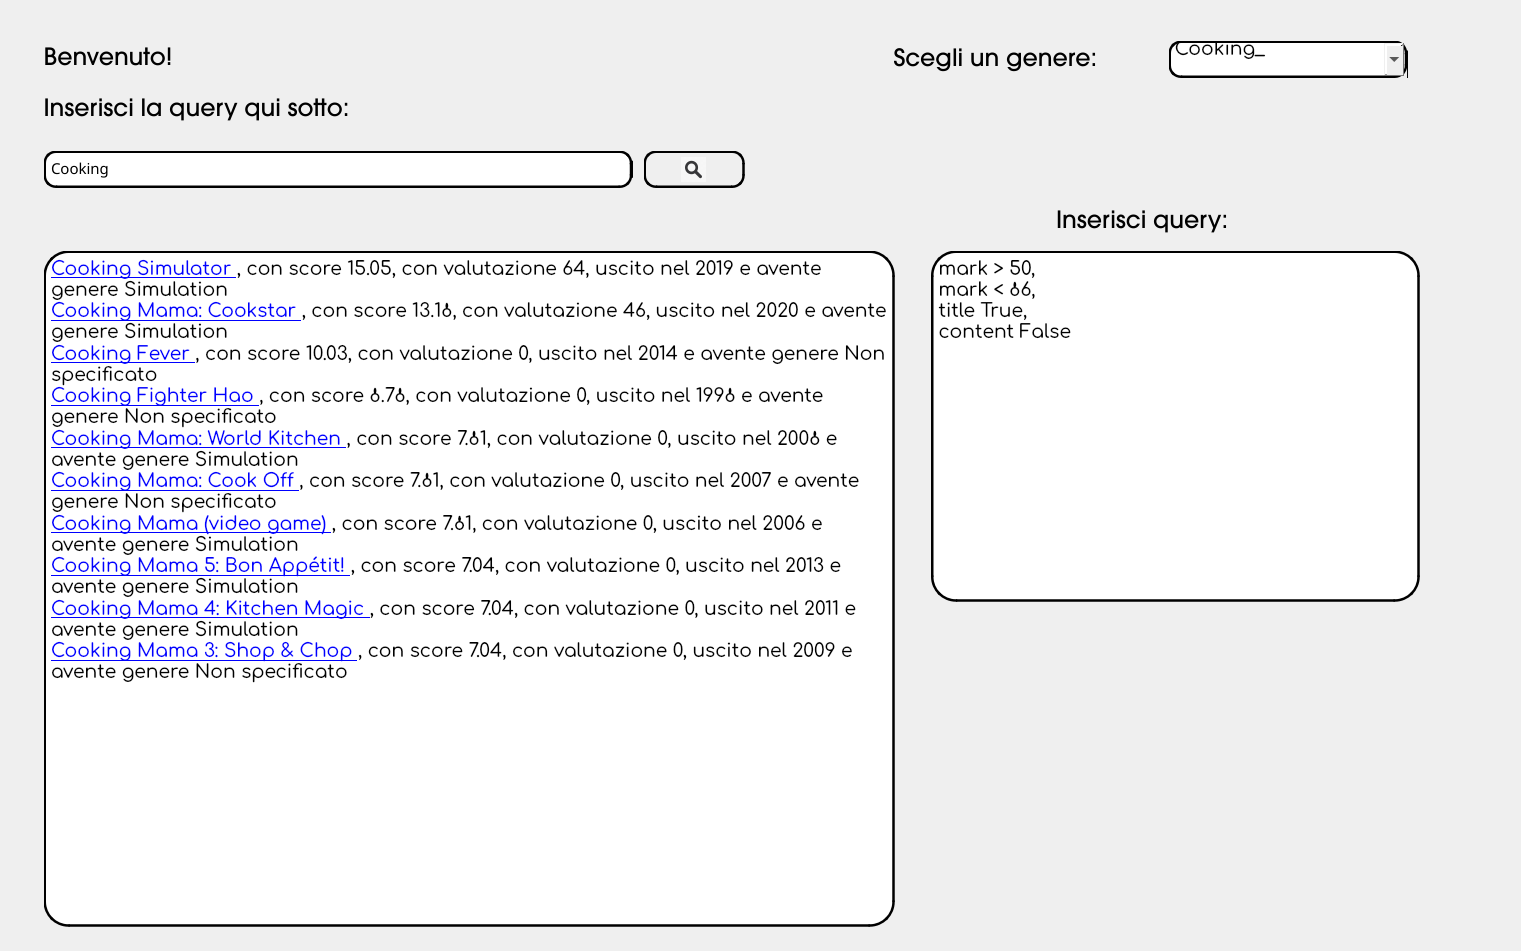
\includegraphics[width=100mm]{Immagini/Image6.png} \\
\textbf{Tempo di esecuzione:} 0.01911s \\
\textbf{Correttezza:} 100\% \pagebreak

\paragraph{Query 7} ~ \\ \\

\noindent \textbf{Keywords: } legends \\
\textbf{Filters: } \{ \\ \\
\indent content False, \\
\indent mark > 70 \\
\} \\\\

\noindent 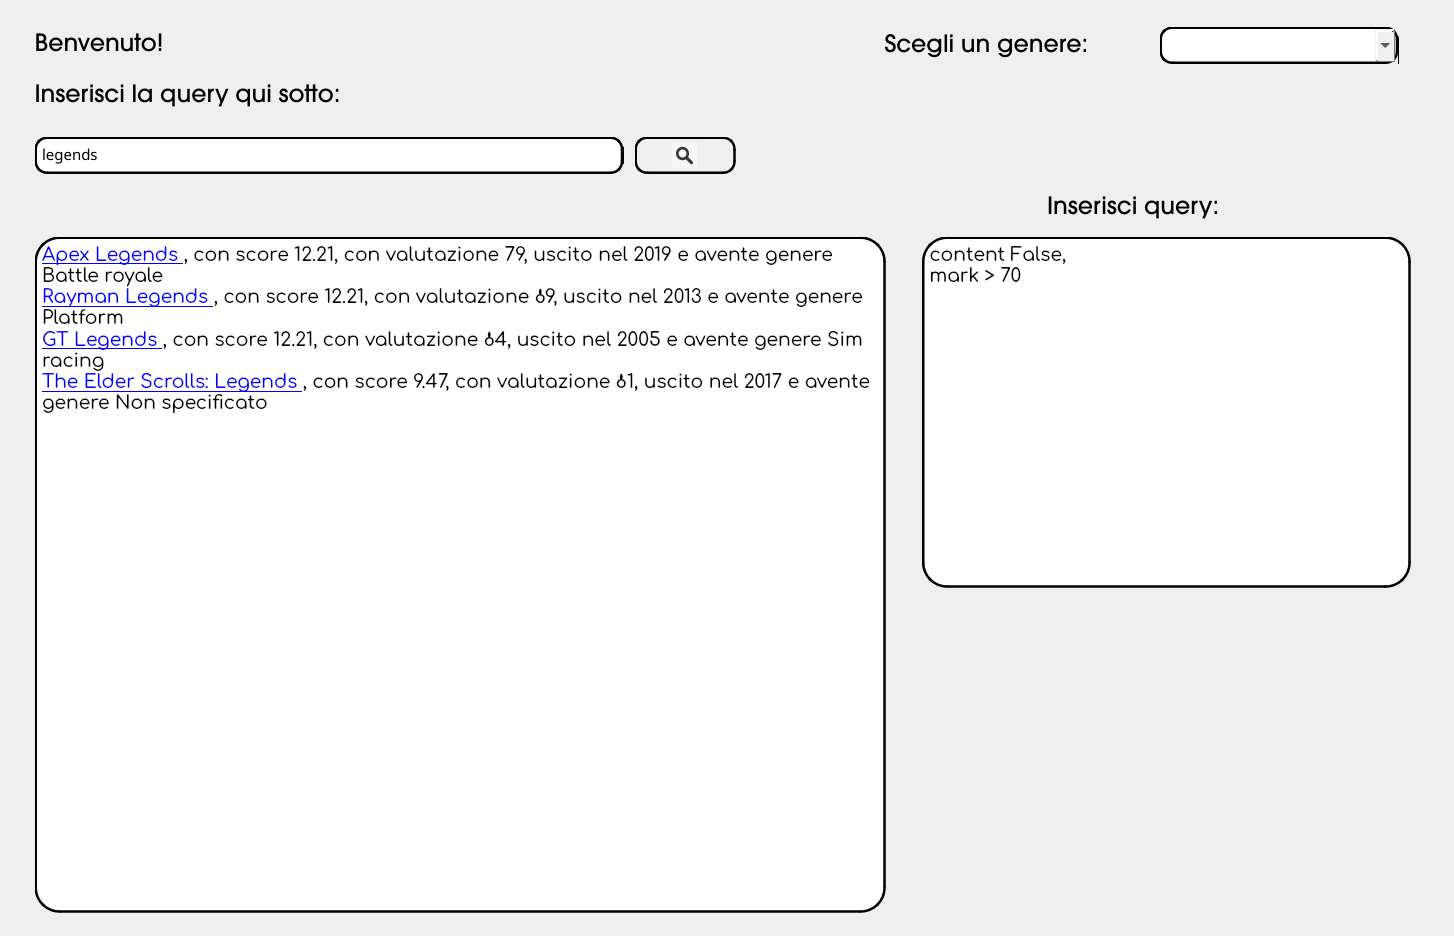
\includegraphics[width=100mm]{Immagini/Image7.png} \\
\textbf{Tempo di esecuzione:} 0.010648 \\
\textbf{Correttezza:} 100\% \pagebreak

\paragraph{Query 8} ~ \\ \\

\noindent \textbf{Keywords: } god war \\
\textbf{Filters: } \{ \\ \\
\indent year > 2000 \\
\} \\\\

\noindent 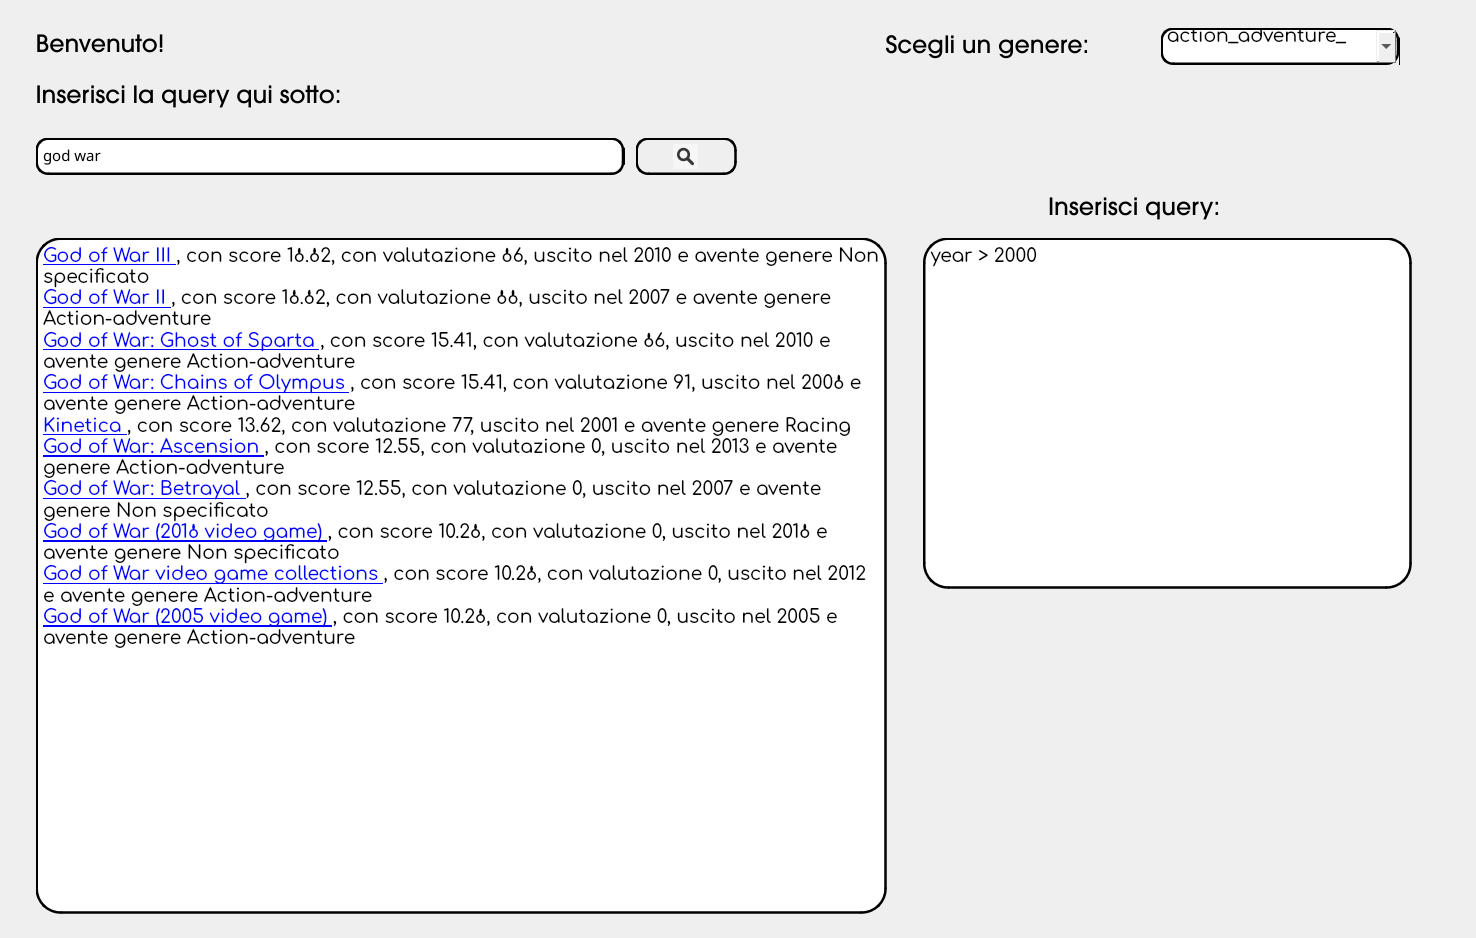
\includegraphics[width=100mm]{Immagini/Image8.png} \\
\textbf{Tempo di esecuzione:} 0.023214 \\
\textbf{Correttezza:} 100\% \pagebreak

\paragraph{Query 9} ~ \\ \\

\noindent \textbf{Keywords: } fifa \\
\textbf{Filters: } \{ \\ \\
\indent mark > 40, \\
\indent year > 2010, \\
\indent year < 2021 \\
\} \\\\

\noindent 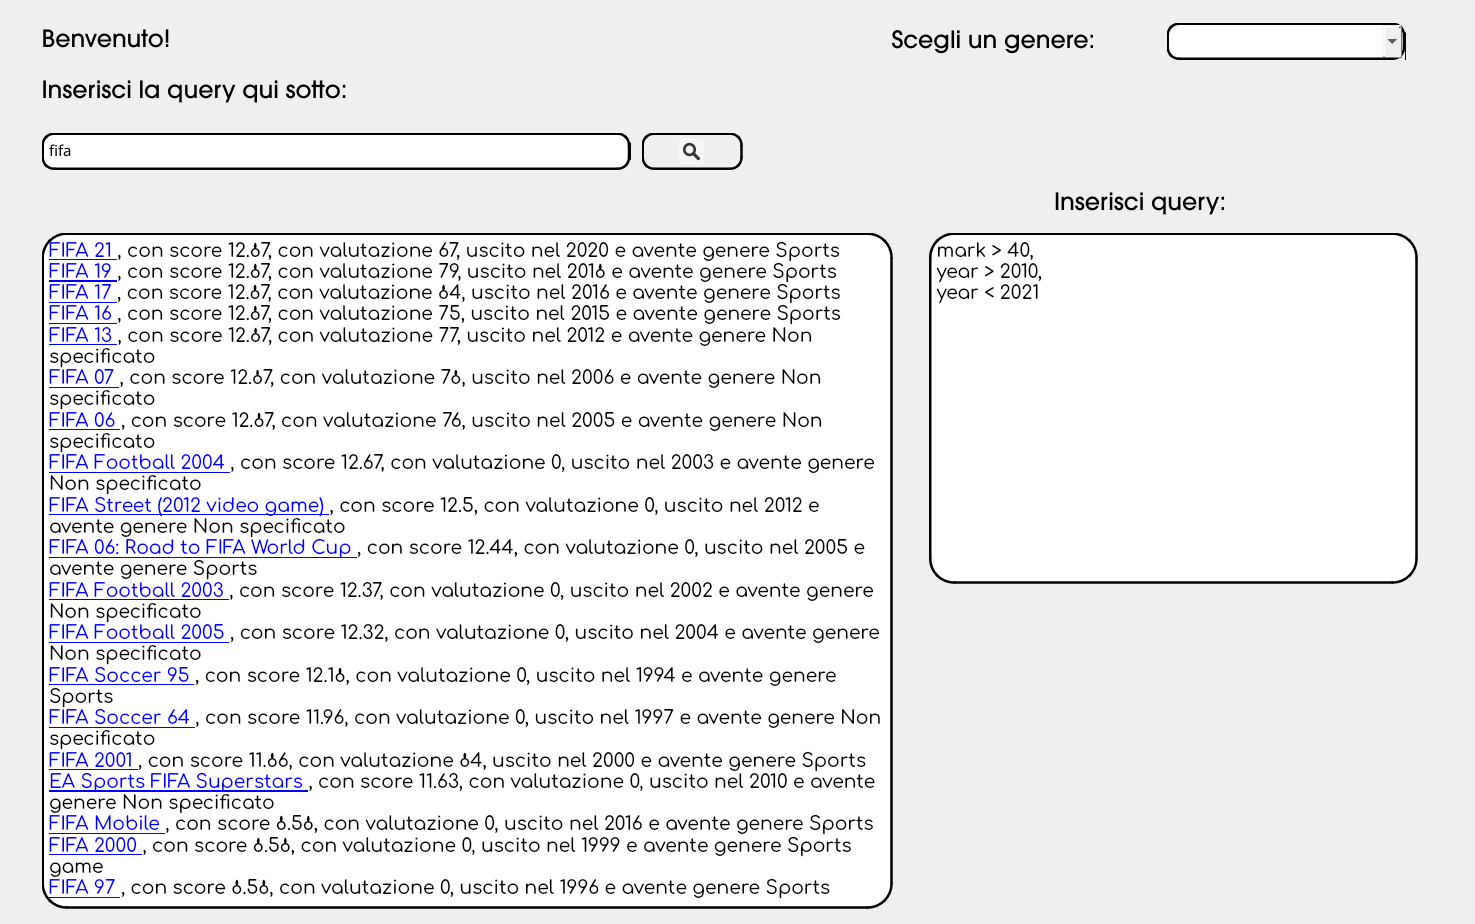
\includegraphics[width=100mm]{Immagini/Image9.png} \\
\textbf{Tempo di esecuzione:} 0.003395 \\
\textbf{Correttezza:} 100\% \pagebreak

\paragraph{Query 10} ~ \\ \\

\noindent \textbf{Keywords: } call duty \\
\textbf{Filters: } \{ \\ \\
\indent mark < 80, \\
\indent title True \\
\} \\\\

\noindent 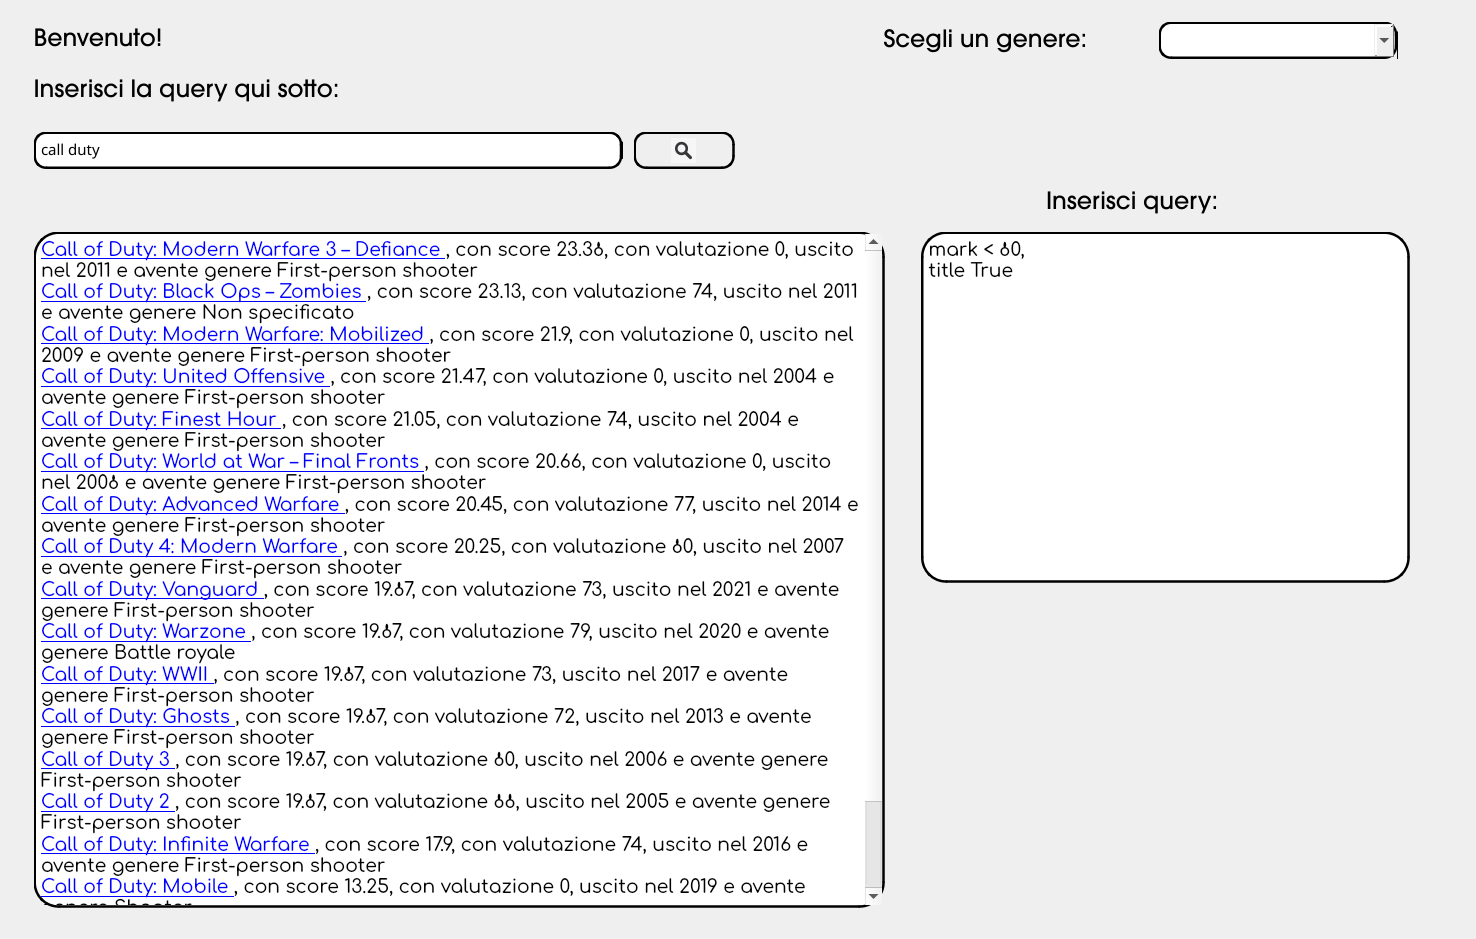
\includegraphics[width=100mm]{Immagini/Image10.png} \\
\textbf{Tempo di esecuzione:} 0.037382 \\
\textbf{Correttezza:} 100\% \pagebreak


\end{document}
